% Background
Learning-based locomotion control methods for quadruped robots have achieved remarkable results in recent years~\cite{xie2021dynamics, tan2018sim, kumar2021rma, nahrendra2023dreamwaq, margolis2023walk, long2024him}.
To adapt to various wild environments, these methods collected large amounts of data in massive parallel simulators with extensive dynamics variations via domain randomization~\cite{tobin2017domain}.
This data-driven paradigm allows RL-based robots to adapt to realistic terrain and unseen disturbances.

% Challenges
While domain randomization is a widely used technique to improve the robustness of robot policies, previous studies~\cite{pmlr-v100-mehta20a, tiboni2023doraemon} have shown that it often sacrifices optimality, resulting in conservative behaviors.
For instance, when trained with large payload variations, the learned policy tends to maintain a lower base height rather than achieve the target height specified in the reward function.
This example reveals that the robustness achieved through domain randomization essentially comes at the cost of compromising certain task objectives under unknown changes.
Consequently, it becomes difficult to consistently meet high task standards, which limits the applicability of domain randomization in complex tasks, particularly those requiring high accuracy.

\begin{figure}[h]
    \centering
    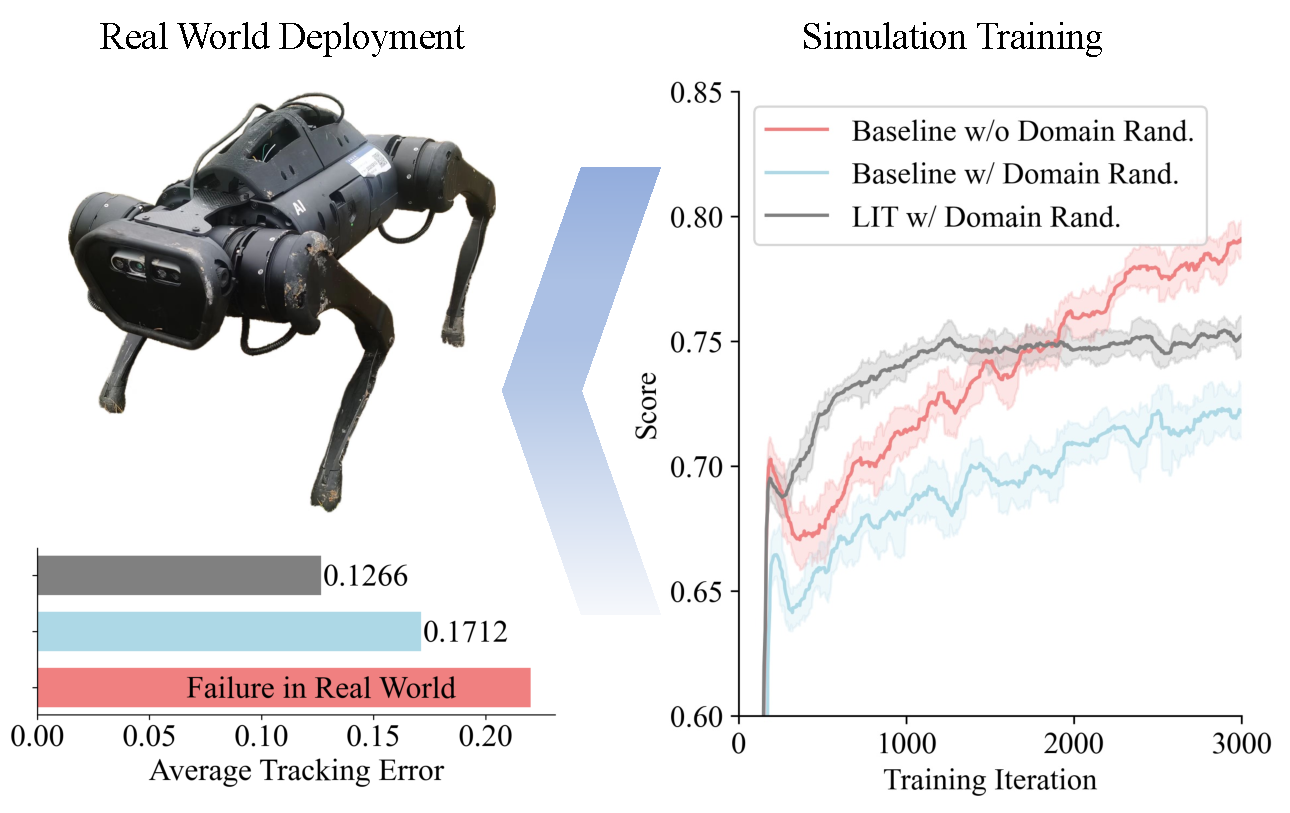
\includegraphics[width=1.0\linewidth]{fig/intro.pdf}
    \caption{\textbf{Proposed LIT has lower tracking error than baseline.} For current RL-based locomotion paradigms (Baseline), domain randomization trades optimality for robustness.}
    \label{fig:intro}
    \vspace{-0.2in}
\end{figure}

% Why 
% This phenomenon is caused by the large amount of random disturbances introduced by domain randomization, which greatly increases the exploration space of RL policy training.
% Furthermore, the environment is modeled as a Partially Observable Markov Decision Process (POMDP)~\cite{spaan2012partially, kurniawati2022partially},  the agent lacks full access to all the perturbed environmental parameters.
% This partial observability forces the policy to adopt conservative behaviors to hedge against potential worst-case scenarios.


% Why Reference
To mitigate this problem, we require a method that can maintain task standards without compromising adaptability under disturbances.  
A key element for enabling robots to recover from unknown perturbations is the explicit identification of the goal that the policy should adapt to. 
This aligns with the control-theoretic perspective, particularly classical disturbance rejection control, where reference signals are used to compute counteractions that cancel perturbation effects
These reference signals define the desired system behavior and represent the performance the controller seeks to preserve despite disturbances.
In RL policy training, however, such references are only implicitly encoded in the reward functions, and no explicit goal-oriented guidance is provided.
Inspired by disturbance rejection control, we therefore propose to supply explicit motion references in RL policy learning.
These references not only provide a clearer objective for training, enabling the policy to learn to resist disturbances and track desired motions, but also deliver richer guidance for policy inference.

% Motivation
Normally, it is straightforward to train a policy in simulation under a fixed set of environmental parameters without any randomization.
Although such a policy cannot be directly deployed in reality due to limited robustness, it can still serve as a reference motion to guide both policy training and inference. Alternatively speaking, a well-trained policy in an ideal simulation can be leveraged to generate goal information that assists the deployed policy in making better decisions. 
To this end, we propose \textbf{LIT} (\textbf{L}earning with \textbf{I}magined \textbf{T}ransition), a two-stage framework training paradigm that enables the learning of robust locomotion policies from ideal motion. 
By introducing “ideal” actions and transitions, the policy could generate actions that are better aligned with nominal dynamics under disturbances (as illustrated by the gray line in Fig.~\ref{fig:intro}), thereby enabling more robust and accurate task execution.

% Framework Overview
Specifically, we reconstruct a learnable dynamics model to approximate transition propagation, obtained from a non-perturbative simulation environment together with an ideal policy. 
These provide reference actions and next-step ideal observations for policy training and inference, guiding the policy toward robust locomotion even under external disturbances.
To achieve this, we incorporate ideal transitions into the policy input while continuing to optimize the policy in an RL manner.
This approach not only improves training efficiency but also enhances the generalization capability of the locomotion policy. 
However, the predicted observation from the dynamics model and ideal policy may become ineffective in Out-of-Distribution (OOD) scenarios. 
If we include it in the optimization objective, it may lead to a training crash or non-convergence.
To address this, we designed an adjustment mechanism of the dynamics model to mitigate the negative impact of OOD observation during policy learning.

% Contribution
In summary, the contributions of our work are as follows:

$\bullet$ We propose \textbf{LIT}, a two-stage RL-based locomotion paradigm that consists of motion reference learning and robust policy learning, leveraging ideal transitions obtained through joint training of the policy and dynamics model in a non-perturbative simulation environment.

$\bullet$ We design an adjustment mechanism to mitigate the adverse effects of dynamics model errors when encountering out-of-distribution (OOD) observations, ensuring efficient and stable policy training.

$\bullet$ We conduct extensive experiments and ablations in both simulators and real-world scenarios. The empirical results demonstrate that LIT improves training efficiency and significantly enhances quadruped locomotion performance under unknown disturbances.